% Options for packages loaded elsewhere
\PassOptionsToPackage{unicode}{hyperref}
\PassOptionsToPackage{hyphens}{url}
%
\documentclass[
]{book}
\usepackage{lmodern}
\usepackage{amssymb,amsmath}
\usepackage{ifxetex,ifluatex}
\ifnum 0\ifxetex 1\fi\ifluatex 1\fi=0 % if pdftex
  \usepackage[T1]{fontenc}
  \usepackage[utf8]{inputenc}
  \usepackage{textcomp} % provide euro and other symbols
\else % if luatex or xetex
  \usepackage{unicode-math}
  \defaultfontfeatures{Scale=MatchLowercase}
  \defaultfontfeatures[\rmfamily]{Ligatures=TeX,Scale=1}
\fi
% Use upquote if available, for straight quotes in verbatim environments
\IfFileExists{upquote.sty}{\usepackage{upquote}}{}
\IfFileExists{microtype.sty}{% use microtype if available
  \usepackage[]{microtype}
  \UseMicrotypeSet[protrusion]{basicmath} % disable protrusion for tt fonts
}{}
\makeatletter
\@ifundefined{KOMAClassName}{% if non-KOMA class
  \IfFileExists{parskip.sty}{%
    \usepackage{parskip}
  }{% else
    \setlength{\parindent}{0pt}
    \setlength{\parskip}{6pt plus 2pt minus 1pt}}
}{% if KOMA class
  \KOMAoptions{parskip=half}}
\makeatother
\usepackage{xcolor}
\IfFileExists{xurl.sty}{\usepackage{xurl}}{} % add URL line breaks if available
\IfFileExists{bookmark.sty}{\usepackage{bookmark}}{\usepackage{hyperref}}
\hypersetup{
  pdftitle={IDA Introduktion til R},
  pdfauthor={Tue Hellstern},
  hidelinks,
  pdfcreator={LaTeX via pandoc}}
\urlstyle{same} % disable monospaced font for URLs
\usepackage{longtable,booktabs}
% Correct order of tables after \paragraph or \subparagraph
\usepackage{etoolbox}
\makeatletter
\patchcmd\longtable{\par}{\if@noskipsec\mbox{}\fi\par}{}{}
\makeatother
% Allow footnotes in longtable head/foot
\IfFileExists{footnotehyper.sty}{\usepackage{footnotehyper}}{\usepackage{footnote}}
\makesavenoteenv{longtable}
\usepackage{graphicx,grffile}
\makeatletter
\def\maxwidth{\ifdim\Gin@nat@width>\linewidth\linewidth\else\Gin@nat@width\fi}
\def\maxheight{\ifdim\Gin@nat@height>\textheight\textheight\else\Gin@nat@height\fi}
\makeatother
% Scale images if necessary, so that they will not overflow the page
% margins by default, and it is still possible to overwrite the defaults
% using explicit options in \includegraphics[width, height, ...]{}
\setkeys{Gin}{width=\maxwidth,height=\maxheight,keepaspectratio}
% Set default figure placement to htbp
\makeatletter
\def\fps@figure{htbp}
\makeatother
\setlength{\emergencystretch}{3em} % prevent overfull lines
\providecommand{\tightlist}{%
  \setlength{\itemsep}{0pt}\setlength{\parskip}{0pt}}
\setcounter{secnumdepth}{5}
\usepackage{booktabs}
\usepackage{amsthm}
\makeatletter
\def\thm@space@setup{%
  \thm@preskip=8pt plus 2pt minus 4pt
  \thm@postskip=\thm@preskip
}
\makeatother
\usepackage[]{natbib}
\bibliographystyle{apalike}

\title{IDA Introduktion til R}
\author{Tue Hellstern}
\date{2020-04-19}

\begin{document}
\maketitle

{
\setcounter{tocdepth}{1}
\tableofcontents
}
\hypertarget{webinar}{%
\chapter{Webinar}\label{webinar}}

Webinar den 22-04-2020

Kl. 19:00

Tue Hellstern

Jelgreen Consult

\hypertarget{intro}{%
\chapter{Introduktion}\label{intro}}

\hypertarget{R_RStudio}{%
\chapter{R og RStudio}\label{R_RStudio}}

Du skal have installeret R og det IDE udviklingsmiljø, der hedder RStudio, begge er open source og begge findes til Mac, Linux og Windows.

\hypertarget{r}{%
\section{R}\label{r}}

Du skal downloade R fra
https://cran.r-project.org
Du skal her vælge den version, der passer til din computer -- Linux, OS X (Mac) eller Windows.
Der er vejledninger for de forskellige installationer på www siden.

\hypertarget{rstudio}{%
\section{RStudio}\label{rstudio}}

Når R er installeret, kan du bruge det, men for at gøre det nemmere bruger vi et udviklingsmiljø, der hedder RStudio. Rstudio findes i flere forskellige versioner, den du skal bruge er \emph{RStudio Desktop Open Source License}

Som du finder her: https://www.rstudio.com/products/rstudio/download/
Du skal her vælge den version, der passer til din computer.

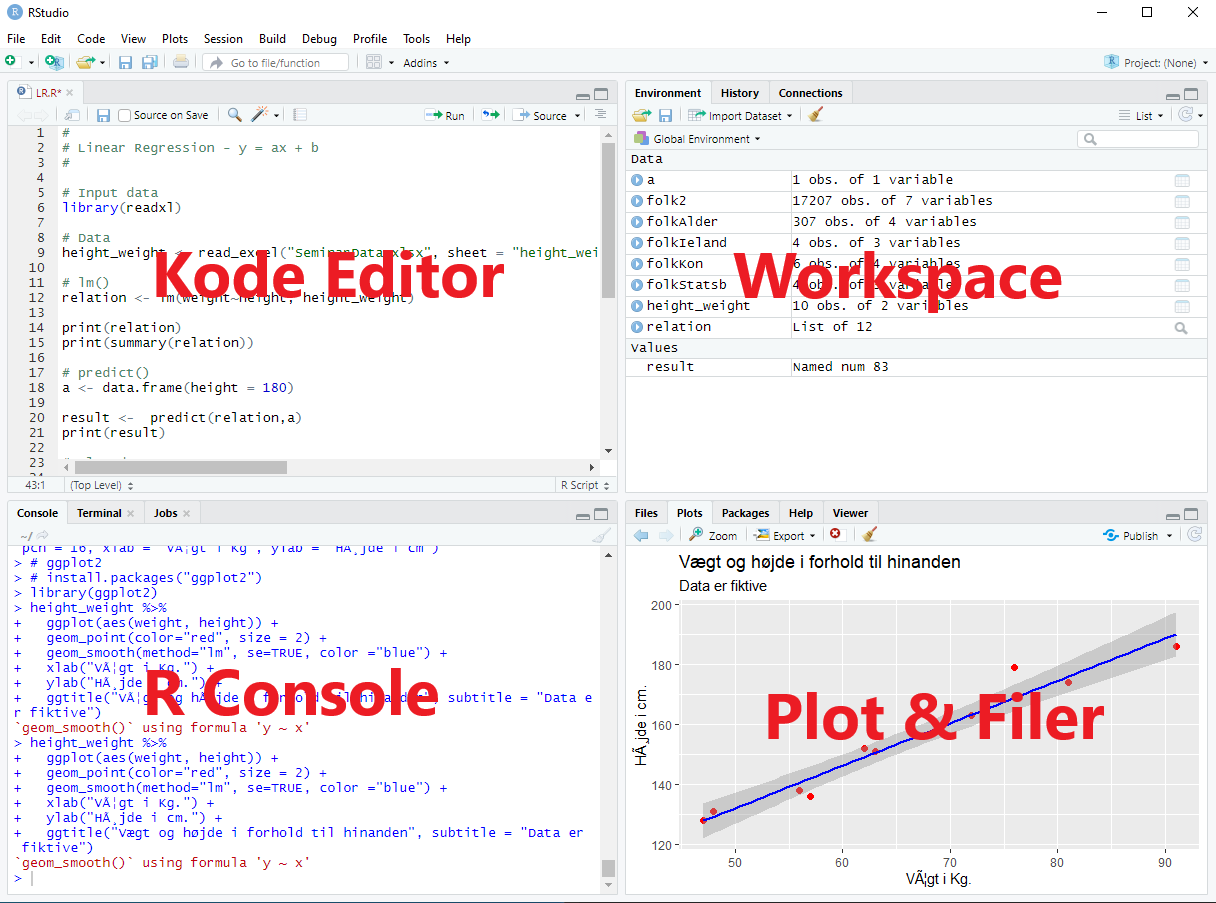
\includegraphics{img/rstudio_editor.png}

\hypertarget{grund}{%
\chapter{Grundlæggende R}\label{grund}}

Som alle andre programmeringssprog har R nogle forskellige regler for, hvordan koden skal bygges op -- altså syntaksen for R.

\hypertarget{navne}{%
\section{Navne}\label{navne}}

''Navne'' i R skal overholde nogle regler:

\begin{itemize}
\tightlist
\item
  Bogstaver -- a til z -- store og små. Du kan ikke bruge de danske tegn æøå
\item
  Tal
\item
  Tegnene ''.'' og ''\_''. Altså ikke mellemrum eller bindestreg
\item
  Et navn kan ikke starte med et Tal, men skal starte med et bogstav eller et gyldigt tegn
\item
  R er case-sensitiv. Der er forskel på store og små bogstaver
\end{itemize}

\hypertarget{variable-objekter}{%
\chapter{Variable / Objekter}\label{variable-objekter}}

Alt hvad du kommer til at bruge i R vil blive gemt i Objekter, det kan være et enkelt tal eller et helt datasæt.
I R skal du bruge ''\textless-'' for at gemme en værdi i et objekt. Mange andre programmeringssprog bruger her ''=''.

´´´
2 + 2 \# Beregn
1:100 \# printer 1 til 100
print(``Hej med dig'')

x \textless- 2 \# Tildel x værdien 2
x * 2
x * x
x + x
x \# Viser værdien af x

y \textless- c(6, 7, 8, 9, 10) \# Gemmer 6 til 10 i variablen y
\# c() står for concatenate eller combine - Giver en vektor

x + y \# x lagt sammen med y
y
x * 2 \# Ganger alle elementer i x med 2 - LOOP uden at være et LOOP ?

ls() \# Vis / List alle objekter
´´´

\hypertarget{funktioner}{%
\section{Funktioner}\label{funktioner}}

R har de sammen funktioner som du måske kender fra Excel eller andre programeringssprog

´´´
length(y) \# Antallet af numre i vektoren
min(y) \# Minimumsværdien
max(y) \# Maksimumværdien
median(y) \# Medianen
sum(y) \# Summen
mean(y) \# Gennemsnittet
var(y) \# Variansen
sd(y) \# Standardafvigelsen
´´´

\hypertarget{logiske-operatorer}{%
\section{Logiske operatorer}\label{logiske-operatorer}}

Meget af det du kommer til at arbejde med i R, vil kræve en eller anden form for logisk operator. Med en logisk operator finder du ud af om et udsagn er Sandt eller Falsk.

´´´
x == 2 \# ``=='' betyder ``lig med''
x != 2 \# ``!='' betyder ``ikke lig med''
x \textless{} 1 \# ``\textless{}'' betyder ``mindre end''
x \textgreater{} 1 \# ``\textgreater{}'' betyder ``større end''
x \textless= 2 \# ``\textless='' betyder "mindre eller lig med
´´´

\emph{Husk, at dette også gælder for de mapper, du arbejder med.}

\hypertarget{hjuxe6lp}{%
\section{Hjælp}\label{hjuxe6lp}}

Du kan få hjælp direkte i R ved at bruge nedstående kommandoer:

´´´
help(``mean'') \# Hjælp til en specifik funktion - mean
help(``plot'')

?mean
?plot

\hypertarget{hjuxe6lp-til-en-specifik-pakke---base-og-tidyverse}{%
\chapter{Hjælp til en specifik pakke - base og tidyverse}\label{hjuxe6lp-til-en-specifik-pakke---base-og-tidyverse}}

help(package = ``base'')
help(package = ``tidyverse'')
´´´

Hjælpen vises i vinduet nederst til højre

\hypertarget{working-directory}{%
\section{Working Directory}\label{working-directory}}

R bruger en mappe som ''Working folder''. Det er nemmere at tilgå filer, der ligger i denne mappe.

´´´
getwd()
setwd(``C:/Users/Tue Hellstern/Documents/GitHub/r\_webinar/r\_kode/webinar\_dag1'')
´´´

\hypertarget{pakker}{%
\chapter{Pakker}\label{pakker}}

Du kan ''tilføje'' funknationalitet til R ved at installere forskellige pakker. Du kan nederst til højre se, hvilke pakker du har installeret.
Det er også her muligt at opdatere de pakker, du har installeret.
Du kan finde en oversigt over de forskellige pakker her: cran.rstudio.com

\hypertarget{installation-af-pakker}{%
\section{Installation af pakker}\label{installation-af-pakker}}

Du kan installere pakker på to måder:

\begin{itemize}
\tightlist
\item
  Via RStudio - GUI
\item
  Via R kode
\end{itemize}

\hypertarget{grafisk}{%
\subsection{Grafisk}\label{grafisk}}

I vinduet nederst til højre kan du klikke på fanen \textbf{Packages} og derefter på knappen \textbf{Install}, du skriver navnet på den eller de pakker du vil installere.

\begin{figure}
\centering
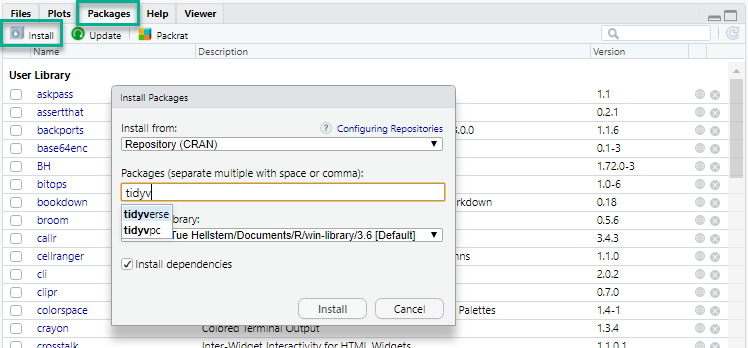
\includegraphics{img/pakker.png}
\caption{Pakker}
\end{figure}

Det er også muligt at opdatere dine pakker vi knappen \textbf{Update}

I sammme vindue kan du også se hvilke pakker der er i \emph{brug}.

\hypertarget{kode}{%
\subsection{Kode}\label{kode}}

Det er nemt at installere og bruge pakker via kode:

\begin{verbatim}
library()                     # Pakker der er på din computer
install.packages("ggplot2")   # install
library(dplyr)                # load

update.packages("tidyverse")  # Update
remove.packages("tidyverse")  # Fjern
\end{verbatim}

\hypertarget{data}{%
\chapter{Data}\label{data}}

For at arbejde med data skal de importeres ind i R. Det er simpelt, hvis de filer der skal importeres ligger i R's aktive bibliotek. Det er en god ide at organisere dine data inden de importeres, hvilket der findes mange gode værktøjer til.
Du kan i RStudio vælge mellem at bruge den grafiske brugerflade (GUI) eller skrive den kode, du vil bruge til importen.

\hypertarget{grafisk-gui}{%
\section{Grafisk (GUI)}\label{grafisk-gui}}

\hypertarget{kode-1}{%
\section{Kode}\label{kode-1}}

\hypertarget{plots}{%
\chapter{Plots}\label{plots}}

\hypertarget{shiny}{%
\chapter{Demo Shiny}\label{shiny}}

Når du har lavet en ''analyse'' i R vil et tit være en fordel at kunne dele denne med andre, det kan du gøre ved at sende den dit R script og data, men det er nok ikke den mest brugervenlige måde.
En anden ulighed er vise det på en webside så det kan tilgås via en browser. Det kan du opnå via en R pakke der hedder shiny.
Du kan finde en del eksempler på løsninger oprettet i shiny her: shiny.rstudio.com/gallery/\#demos

Det er også muligt at afvikle de 11 eksempler der følger med shiny på følgende måde:

\begin{verbatim}
# Shiny eksempler
runExample("01_hello")
runExample("02_text")
runExample("03_reactivity")
runExample("04_mpg")
runExample("05_sliders")
runExample("06_tabsets")
runExample("07_widgets")
runExample("08_html")
runExample("09_upload")
runExample("10_download")
runExample("11_timer")
\end{verbatim}

\hypertarget{struktur-af-en-shiny-app}{%
\section{Struktur af en Shiny app}\label{struktur-af-en-shiny-app}}

En Shimy App er ''samlet'' i et enkelt script app.R som du kan afvikle.
app.R består af tre dele:

\begin{itemize}
\tightlist
\item
  Userinterface (ui.R) - \emph{Her styrer du layout af din applikation}
\item
  Server (server.R) - \emph{Her definere du det der skal til for at opbygge din løsning}
\item
  Kald til shinyApp function - \emph{Her bygges selev løsningen}
\end{itemize}

Du kan oprette en ny shiny App under:
\textbf{File -- New File -- Shiny Web App}
I dette vindue skal du indtaste navnet på din App og placeringen. Du har også mulighed for at vælge mellem og din App skal opdeles i to file, \textbf{ui.R} og \textbf{server.R}, eller om du vil have alt i en fil.

Opdelingen i to filer giver dig de fleste muligheder og en bedre kontrol.

Du får to filer der indeholder en demo løsning som du kan bruge som
udgangspunkt for din egen løsning.

\hypertarget{links}{%
\chapter{Links}\label{links}}

Her er en lille samling af nyttige links, det er på ingen måde en fuldstændig liste -- Brug Google.

\begin{itemize}
\tightlist
\item
  www.rproject.org
\item
  mran.microsoft.com/open
\item
  www.rstudio.com
\item
  support.rstudio.com/hc/en-us/categories/200035113-Documentation
\item
  www.statmethods.net
\end{itemize}

  \bibliography{book.bib,packages.bib}

\end{document}
